\documentclass[final,5p,times,twocolumn]{elsarticle}
\usepackage{amsmath,amssymb}
\usepackage{booktabs}
\usepackage{microtype}
\usepackage{graphicx}
\journal{Materials Letters}

\begin{document}
\begin{frontmatter}

\title{Formula-Invariant Chemical Diversification for Robust Candidate Shortlisting in Oxide Materials Databases}
\author[aff1]{Lu Zhang\corref{cor1}}
\ead{2023003177@mails.cust.edu.cn}
\author[aff2]{Gaoding Zhou}
\address[aff1]{School of Materials Science and Engineering, Changchun University of Science and Technology, Changchun 130022, China}
\address[aff2]{School of Artificial Intelligence, Changchun University of Science and Technology, Changchun 130022, China}
\cortext[cor1]{Corresponding author. Email: 2023003177@mails.cust.edu.cn}

\begin{abstract}
Database screening often ends with a single scalar score, although the final shortlist can change when the same objectives are combined by a different scoring formula. We introduce Formula-Invariant Chemical Diversification (FICD), a post-filter procedure that explicitly treats this scoring-formulation uncertainty before chemical diversification. Stability and band-gap preferences are evaluated with arithmetic, geometric, harmonic, and Chebyshev scalarizations over four non-extreme weight settings. Their rank fingerprints define a scoring-invariance index and cross-family eligibility. A Top-25 quality seed is then diversified only through swaps that do not increase its worst scoring-rule regret. On Materials Project Li--Mn--O and WBM-derived oxygen-containing subsets, the mean nearest-neighbor composition distance increases by 68.2\% and 15.7\%, respectively, while the worst-rule regret does not increase. Leave-one-family-out tests, an independent ElMD distance check, and Materials Project space-group coverage provide validation outside the quantities used by the main ranking. FICD therefore provides a compact quality-first alternative to unconstrained relevance-diversity reranking for pre-experimental materials shortlisting.
\end{abstract}

\begin{keyword}
materials informatics \sep candidate prioritization \sep oxide materials \sep robust ranking \sep chemical diversity \sep band gap
\end{keyword}
\end{frontmatter}

\section{Introduction}
High-throughput resources such as the Materials Project, OQMD, and AFLOW make large-scale computational screening routine \cite{Jain2013,Saal2013,Curtarolo2012}. Materials-informatics frameworks and benchmarks have further improved property prediction and prospective triage \cite{Ward2016,Butler2018,Morgan2020,Dunn2020,Riebesell2025}. Yet a practical issue remains after physical filtering: a small experimental or higher-level-computation budget still requires a shortlist.

A weighted sum is transparent, but its output depends on the chosen utility form. Uncertain preferences have long been studied by multicriteria acceptability analysis \cite{Lahdelma2001}, while relevance-diversity reranking, robust subset selection, and determinantal approaches address redundancy in selected sets \cite{Carbonell1998,Krause2008,Nava2022}. In materials data, composition metrics such as ElMD and redundancy-control methods such as MD-HIT similarly show that chemically repetitive selections can obscure coverage \cite{Hargreaves2020,Li2024}. Recent strong-regret formulations also combine utility guarantees with diversity in generic databases \cite{Guo2025}. Consequently, neither rank aggregation nor diversity selection alone is a sufficient novelty claim.

Here the target is narrower: post-filter materials shortlisting under \emph{scoring-formulation uncertainty}. FICD first identifies candidates supported across distinct scalarization families, then permits chemical diversification only when the seed set's worst cross-formula regret is preserved. ``Formula-invariant'' is therefore operational: reduced sensitivity within a declared family of reasonable scalarizations, not invariance to arbitrary utility functions.

\section{Data and method}
Two oxide pools were used. A Materials Project (MP) Li--Mn--O subset was filtered at $E_{\rm hull}\leq0.05$ eV/atom, and a WBM-derived oxygen-containing subset at $E_{\rm hull}\leq0.08$ eV/atom. After positive-gap and nonmetal admissibility, 208 MP and 45 WBM candidates remained; $K=25$ was used as the common shortlist budget. The WBM subset is used for transferability, not for reproducing the full Matbench Discovery benchmark \cite{Riebesell2025}.

For each admissible pool, stability $S_i$ and band-gap preference $G_i$ were min--max scaled to $[0,1]$, with larger values preferred. Four scalarization families were evaluated at $w\in\{0.4,0.5,0.6,0.7\}$:
\begin{align}
U_i^{A}&=wS_i+(1-w)G_i,\\
U_i^{G}&=S_i^wG_i^{1-w},\\
U_i^{H}&=\left(w/S_i+(1-w)/G_i\right)^{-1},\\
U_i^{T}&=1-\max\{w(1-S_i),(1-w)(1-G_i)\}.
\end{align}
Thus each material has 16 ranks. For rule $\ell$, the rank desirability is $q_{i\ell}=1-(r_{i\ell}-1)/N$. Its geometric consensus and log-rank dispersion are
\begin{equation}
C_i=\exp\!\left(\overline{\ln q_i}\right),\qquad
V_i={\rm std}(\ln q_i),\qquad
I_i=C_i e^{-V_i}.
\end{equation}
$I_i$ is the scoring-invariance index (SII). Let $F_i\in\{0,1,2,3,4\}$ count the scalarization families in which candidate $i$ enters at least one Top-$K$ list. Candidates with $F_i\geq2$ form the eligible reservoir, and
\begin{equation}
Q_i=\sqrt{I_iF_i/4}
\end{equation}
combines rank invariance and cross-family support without a fitted mixing coefficient. The Top-$K$ candidates by $Q_i$ define the quality seed $A_0$.

For a selected set $A$, rule-specific regret is
\begin{equation}
r_{\ell}(A)=\overline{q}_{\ell}^{\,\mathrm{Top}K}-\frac{1}{K}\sum_{i\in A}q_{i\ell},\qquad
R(A)=\max_{\ell} r_{\ell}(A).
\end{equation}
FICD then performs best-improvement one-for-one swaps within the eligible reservoir. A swap is accepted only if $R(A')\leq R(A_0)$ and it strictly increases
\begin{equation}
d_{\rm NN}(A)=\frac{1}{K}\sum_{i\in A}\min_{j\in A\setminus i} d(i,j).
\end{equation}
The primary distance is total variation between oxygen-excluded, $L_1$-normalized cation fractions, $d(i,j)=\tfrac12\lVert\mathbf c_i-\mathbf c_j\rVert_1$. ElMD with the modified-Pettifor basis \cite{Hargreaves2020} was used only as an independent distance validation.

\begin{figure}[t]
\centering
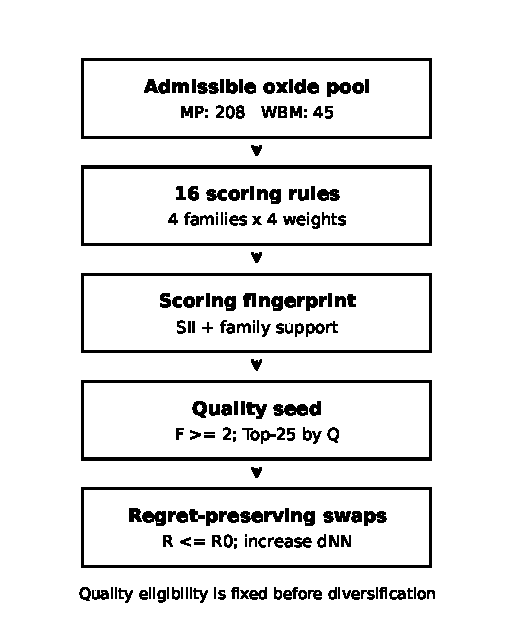
\includegraphics[width=\columnwidth]{figures/figure1_method.pdf}
\caption{FICD separates cross-formula quality eligibility from regret-preserving chemical diversification.}
\label{fig:method}
\end{figure}

\begin{figure*}[t]
\centering
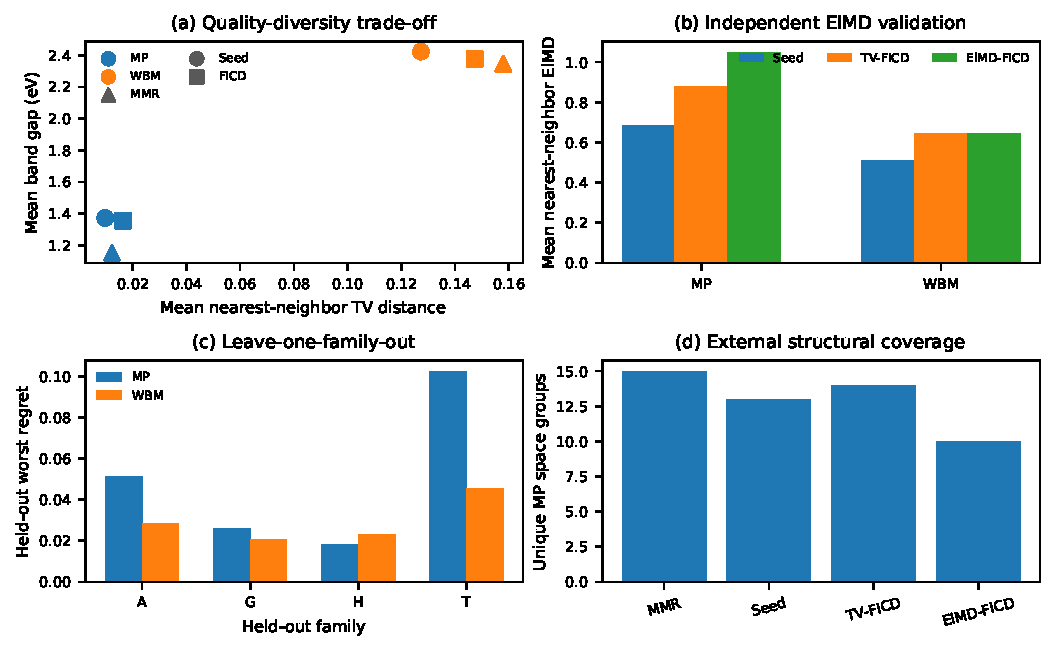
\includegraphics[width=0.97\textwidth]{figures/figure2_validation.pdf}
\caption{Validation of the frozen FICD procedure. (a) Quality--diversity comparison. (b) Independent ElMD nearest-neighbor diversity. (c) Worst regret on a scalarization family excluded from construction. (d) External MP space-group coverage.}
\label{fig:validation}
\end{figure*}

\section{Results and discussion}
Table~\ref{tab:main} compares the frozen FICD result with its quality seed and a maximal-marginal-relevance (MMR) baseline. On MP, one admissible swap increases $d_{\rm NN}$ from 0.00978 to 0.01644 (68.2\%) while the mean band gap changes from 1.372 to 1.356 eV (1.2\% decrease); worst-rule regret slightly decreases from 0.08750 to 0.08731. On WBM, $d_{\rm NN}$ rises from 0.1273 to 0.1473 (15.7\%), the mean band gap changes from 2.422 to 2.376 eV (1.9\%), and worst-rule regret decreases from 0.04444 to 0.04356. Compared with MMR, FICD has higher mean band gap and substantially lower worst-rule regret in both datasets; WBM MMR retains a modest diversity advantage.

\begin{table*}[t]
\centering
\caption{Top-25 shortlist comparison. $d_{\rm NN}$ uses cation-fraction total-variation distance.}
\label{tab:main}
\small
\begin{tabular}{llcccc}
\toprule
Dataset & Method & $\overline{E_g}$ (eV) & $\overline{E}_{\rm hull}$ (eV/atom) & $d_{\rm NN}$ & Worst-rule regret \\
\midrule
MP & MMR & 1.152 & 0.01265 & 0.01229 & 0.28789 \\
MP & Cross-family $Q$ seed & 1.372 & 0.01820 & 0.00978 & 0.08750 \\
MP & FICD & 1.356 & 0.01806 & 0.01644 & 0.08731 \\
WBM & MMR & 2.345 & 0.02986 & 0.15800 & 0.05911 \\
WBM & Cross-family $Q$ seed & 2.422 & 0.03104 & 0.12733 & 0.04444 \\
WBM & FICD & 2.376 & 0.03040 & 0.14733 & 0.04356 \\
\bottomrule
\end{tabular}
\end{table*}

Three checks were used to test whether these gains were specific to the construction choices. First, rebuilding the diversification objective with official ElMD increased MP mean nearest-neighbor ElMD from 0.683 for the seed to 1.050; the ElMD-selected shortlist retained 84\% overlap with the TV-selected FICD set and had worst-rule regret 0.08596. For WBM, TV- and ElMD-objective FICD produced the same Top-25. Second, leave-one-family-out construction used only three scalarization families and evaluated the fourth only after selection. Held-out worst regret remained below 0.046 on WBM; the largest value was 0.103 on MP when Chebyshev scoring was excluded from construction. This is evidence for reduced formula sensitivity, while also showing that the invariance is not absolute.

Third, MP crystal system and space group were never used for ranking. TV-FICD increased unique space groups from 13 in the quality seed to 14 and the effective number $\exp(H)$ from 9.98 to 11.12. MMR reached 15 space groups, whereas ElMD-objective FICD reached only 10, showing that a chemically sophisticated distance does not automatically maximize structural coverage. Family-support sensitivity also argues against threshold cherry-picking: MP thresholds of one and two supported families give the same result, as do WBM thresholds one through three; requiring all four families leaves only 20 MP candidates and is infeasible for $K=25$.

The main limitation is that both objectives are database descriptors; FICD prioritizes follow-up calculations or experiments rather than proving synthesis or device performance. It also depends on a declared scalarization family and a composition distance. The LOFO and ElMD tests quantify these dependencies instead of treating them as absent.

\section{Conclusions}
FICD converts scoring-formulation uncertainty into an explicit quality constraint before diversity is optimized. Across two oxide pools, chemical separation increased without increasing worst-rule regret, and the behavior persisted under held-out scoring families and an independent composition metric. The method is intended as a lightweight post-filter layer for fixed-budget, pre-experimental shortlisting.

\section*{Acknowledgements}
The authors thank Yunlong Jiang, School of Materials Science and Engineering, Changchun University of Science and Technology, for supervision and project guidance.

\section*{Data availability}
The processed candidate tables, validation outputs, figures, and reproducibility scripts supporting this study are archived in Zenodo. The final DOI will be inserted before online submission: \textbf{[ZENODO DOI PENDING]}.

\section*{Declaration of competing interest}
The authors declare no competing financial interests.

\section*{Declaration of generative AI and AI-assisted technologies in manuscript preparation}
During the preparation of this work, the authors used ChatGPT by OpenAI and DeepSeek for language polishing, manuscript restructuring, LaTeX formatting, and preparation of submission-related documents. The authors reviewed and edited the content as needed and take full responsibility for the content of the manuscript.

\begin{thebibliography}{99}
\bibitem{Jain2013} A. Jain et al., APL Mater. 1 (2013) 011002. doi:10.1063/1.4812323.
\bibitem{Saal2013} J.E. Saal et al., JOM 65 (2013) 1501--1509. doi:10.1007/s11837-013-0755-4.
\bibitem{Curtarolo2012} S. Curtarolo et al., Comput. Mater. Sci. 58 (2012) 218--226. doi:10.1016/j.commatsci.2012.02.005.
\bibitem{Ward2016} L. Ward et al., npj Comput. Mater. 2 (2016) 16028. doi:10.1038/npjcompumats.2016.28.
\bibitem{Butler2018} K.T. Butler et al., Nature 559 (2018) 547--555. doi:10.1038/s41586-018-0337-2.
\bibitem{Morgan2020} D. Morgan, R. Jacobs, Annu. Rev. Mater. Res. 50 (2020) 71--103. doi:10.1146/annurev-matsci-070218-010015.
\bibitem{Dunn2020} A. Dunn et al., npj Comput. Mater. 6 (2020) 138. doi:10.1038/s41524-020-00406-3.
\bibitem{Riebesell2025} J. Riebesell et al., Nat. Mach. Intell. 7 (2025) 836--847. doi:10.1038/s42256-025-01055-1.
\bibitem{Carbonell1998} J. Carbonell, J. Goldstein, Proc. SIGIR (1998) 335--336. doi:10.1145/290941.291025.
\bibitem{Lahdelma2001} R. Lahdelma, P. Salminen, Oper. Res. 49 (2001) 444--454. doi:10.1287/opre.49.3.444.11220.
\bibitem{Krause2008} A. Krause et al., J. Mach. Learn. Res. 9 (2008) 2761--2801.
\bibitem{Nava2022} E. Nava et al., Proc. AISTATS, PMLR 151 (2022).
\bibitem{Hargreaves2020} C.J. Hargreaves et al., Chem. Mater. 32 (2020) 10610--10620. doi:10.1021/acs.chemmater.0c03381.
\bibitem{Li2024} Q. Li et al., npj Comput. Mater. 10 (2024) 245. doi:10.1038/s41524-024-01426-z.
\bibitem{Guo2025} H. Guo et al., Theor. Comput. Sci. 1026 (2025) 114986.
\end{thebibliography}
\end{document}
